\documentclass[tikz,border=3pt]{standalone}
\usepackage[utf8]{inputenc}
\usepackage{pgfplots}
\pgfplotsset{compat=1.18}

\definecolor{satblue}{HTML}{0072B2}
\definecolor{unsatorange}{HTML}{D55E00}
\definecolor{timeoutgray}{HTML}{6B7280}
\definecolor{errorpurple}{HTML}{CC79A7}

\begin{document}
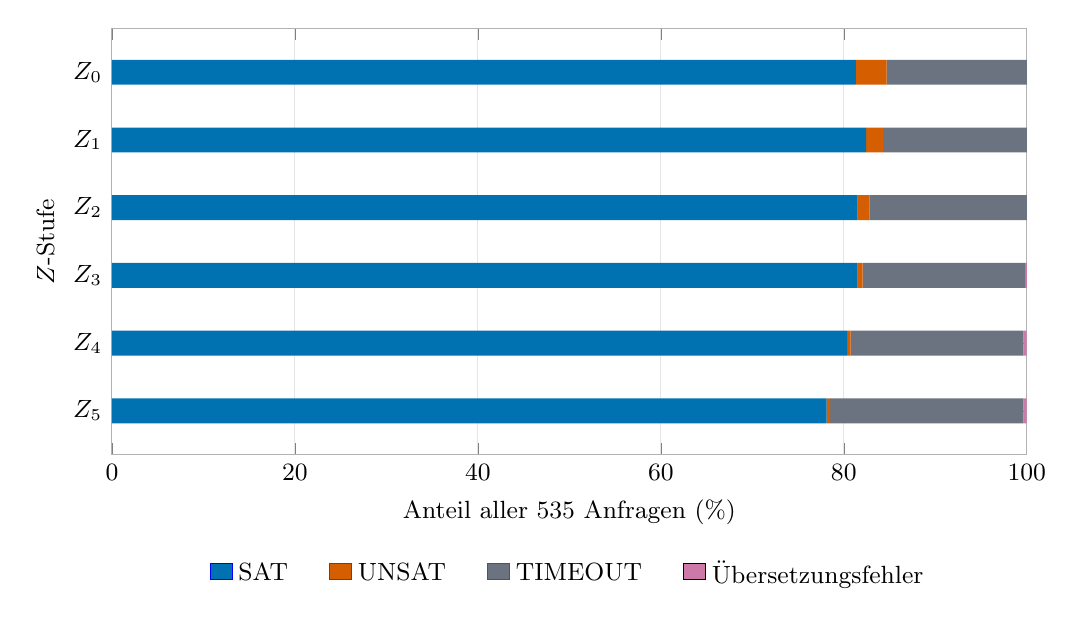
\begin{tikzpicture}
\begin{axis}[
    width=13.2cm,
    height=7.0cm,
    xbar stacked,
    xmin=0,
    xmax=100,
    bar width=9pt,
    symbolic y coords={Z5,Z4,Z3,Z2,Z1,Z0},
    ytick=data,
    yticklabels={$Z_0$,$Z_1$,$Z_2$,$Z_3$,$Z_4$,$Z_5$},
    xlabel={Anteil aller 535 Anfragen (\%)},
    ylabel={$Z$-Stufe},
    xtick={0,20,40,60,80,100},
    grid=major,
    grid style={draw=gray!20},
    axis line style={draw=gray!60},
    tick label style={font=\small},
    label style={font=\small},
    enlarge y limits=0.13,
    legend columns=4,
    legend style={
        at={(0.5,-0.22)},
        anchor=north,
        draw=none,
        font=\small,
        /tikz/every even column/.append style={column sep=0.45cm}
    }
]
\addplot+[draw=none,fill=satblue] coordinates {
    (81.31,Z0) (82.43,Z1) (81.50,Z2) (81.50,Z3) (80.37,Z4) (78.13,Z5)
};
\addplot+[draw=none,fill=unsatorange] coordinates {
    (3.36,Z0) (1.87,Z1) (1.31,Z2) (0.56,Z3) (0.37,Z4) (0.37,Z5)
};
\addplot+[draw=none,fill=timeoutgray] coordinates {
    (15.33,Z0) (15.70,Z1) (17.20,Z2) (17.76,Z3) (18.88,Z4) (21.12,Z5)
};
\addplot+[draw=none,fill=errorpurple] coordinates {
    (0.00,Z0) (0.00,Z1) (0.00,Z2) (0.19,Z3) (0.37,Z4) (0.37,Z5)
};
\legend{SAT,UNSAT,TIMEOUT,Übersetzungsfehler}
\end{axis}
\end{tikzpicture}
\end{document}
